% ============================================================
% APPENDIX
% Overflow from Chapters 4 and 5, preserved in substance but
% moved here to keep the main text reader-friendly.
% ============================================================

\subsection{Accuracy and Efficiency: Full Configuration Table}
\label{app:perf:configs}

\autoref{tab:app:perf:configs} reports accuracy, mean rounds to consensus,
fraction of repetitions hitting the hard cap $T = 15$, and mean vote flips
for all 12 (dataset, topology, $W$) configurations
($R = 50$ repetitions per task, $n = 2{,}500$ repetitions per cell).

\begin{table}[H]
\centering
\small
\begin{tabular}{llccccc}
\toprule
Dataset & Config & Accuracy & Mean rounds & $p_{\mathrm{cap}}$ & Mean flips \\
\midrule
GPQA & fc / $W=1$ & $41.4\,\%$ & $3.87$ & $0.2\,\%$ & $2.98$ \\
     & fc / $W=2$ & $43.1\,\%$ & $3.68$ & $0.2\,\%$ & $2.90$ \\
     & fc / $W=5$ & $42.4\,\%$ & $3.83$ & $0.4\,\%$ & $2.91$ \\
     & star / $W=1$ & $41.8\,\%$ & $4.29$ & $1.0\,\%$ & $3.11$ \\
     & star / $W=2$ & $42.5\,\%$ & $4.23$ & $1.0\,\%$ & $3.77$ \\
     & star / $W=5$ & $42.2\,\%$ & $4.36$ & $1.6\,\%$ & $3.43$ \\
\addlinespace
HiddenBench & fc / $W=1$ & $25.2\,\%$ & $5.18$ & $2.5\,\%$ & $4.27$ \\
            & fc / $W=2$ & $28.2\,\%$ & $4.71$ & $1.0\,\%$ & $3.92$ \\
            & fc / $W=5$ & $25.8\,\%$ & $4.79$ & $2.0\,\%$ & $3.86$ \\
            & star / $W=1$ & $24.5\,\%$ & $7.13$ & $13.3\,\%$ & $4.82$ \\
            & star / $W=2$ & $26.6\,\%$ & $6.48$ & $11.2\,\%$ & $5.22$ \\
            & star / $W=5$ & $26.4\,\%$ & $6.27$ & $10.7\,\%$ & $5.12$ \\
\bottomrule
\end{tabular}
\caption[Accuracy and efficiency by configuration]{Full system performance per configuration
         ($R = 50$, $50$ tasks, $n = 2{,}500$ repetitions per cell).}
\label{tab:app:perf:configs}
\end{table}

\subsection{Accuracy and Efficiency: Rounds vs.\ Accuracy}
\label{app:perf:rounds_acc}

\begin{figure}[H]
  \centering
  \includegraphics[width=0.9\linewidth]{plots/general/fig5_rounds_vs_accuracy.png}
  \caption[Accuracy versus rounds to consensus]{Mean accuracy as a function of rounds to consensus,
           for GPQA (left) and HiddenBench (right).
           Points show means over repetitions reaching each round count
           (minimum $n = 20$).
           All configurations pooled ($N = 15{,}000$ per dataset).}
  \label{fig:app:perf:rounds_acc}
\end{figure}

\subsection{Self-Reinforcement: Supplementary Tables and Figure}
\label{app:sr:supp}

\autoref{tab:sr:overview} reports $p_{\mathrm{SR}}$ and mean slope $\bar\beta$ for
all 12 (dataset, topology, $W$) cells; \autoref{tab:sr:subgroups} breaks the
segment-level slope down by structural condition; \autoref{fig:sr:accuracy} shows
the marginal (pooled) relationship between $\bar\beta$ and task accuracy, whose
near-zero correlation is discussed in \autoref{sec:results:sr}.

\begin{table}[H]
\centering
\small
\begin{tabular}{llcc}
\toprule
Dataset & Topology & $p_{\mathrm{SR}}$ (range over $W$) & $\bar{\beta}$ (range over $W$) \\
\midrule
GPQA        & fc   & 0.763--0.825 & 0.441--0.515 \\
GPQA        & star & 0.733--0.809 & 0.390--0.463 \\
HiddenBench & fc   & 0.839--0.881 & 0.415--0.467 \\
HiddenBench & star & 0.804--0.844 & 0.350--0.373 \\
\bottomrule
\end{tabular}
\caption[Self-reinforcement prevalence and slope by configuration]{$p_{\mathrm{SR}}$ and mean segment slope $\bar\beta$
         (confidence gain / round) per (dataset, topology) configuration,
         range reported over $W \in \{1,2,5\}$.
         $N_{\mathrm{tasks}} = 50$, $R = 50$.}
\label{tab:sr:overview}
\end{table}

\begin{table}[H]
\centering

\small
\begin{tabular}{llrrl}
\toprule
Condition & Group & $n_{\mathrm{segs}}$ & $\bar\beta$ & $p_{\mathrm{SR}}$ \\
\midrule
\multirow{2}{*}{Ceiling}
  & No ceiling   & 115{,}137 & 0.404 & 0.798 \\
  & Ceiling hit  &  18{,}559 & 0.564 & 0.910 \\
\midrule
\multirow{2}{*}{Terminality}
  & Non-terminal &  14{,}341 & 0.262 & 0.682 \\
  & Terminal     & 119{,}355 & 0.445 & 0.829 \\
\midrule
\multirow{2}{*}{Initial correctness}
  & Init wrong majority   & 116{,}400 & 0.410 & 0.809 \\
  & Init correct majority &  17{,}296 & 0.535 & 0.840 \\
\midrule
\multirow{2}{*}{Vote stability}
  & Some agent flipped    & 113{,}660 & 0.380 & 0.796 \\
  & Fully static rep.     &  20{,}036 & 0.685 & 0.908 \\
\midrule
\multirow{5}{*}{Init vote dist.}
  & 4-0-0-0 & 21{,}435 & 0.663 & 0.897 \\
  & 3-1-0-0 & 50{,}286 & 0.412 & 0.824 \\
  & 2-2-0-0 & 26{,}629 & 0.370 & 0.791 \\
  & 2-1-1-0 & 34{,}035 & 0.345 & 0.767 \\
  & 1-1-1-1 &   1{,}311 & 0.308 & 0.656 \\
\bottomrule
\end{tabular}
\caption[Self-reinforcement slope by structural subgroup]{Mean segment slope $\bar\beta$ and $p_{\mathrm{SR}}$ by subgroup
         (all segments pooled across configs, $N = 133{,}696$).
         Pooled segment counts are descriptive; the subgroup orderings are
         confirmed at the task level.}
\label{tab:sr:subgroups}
\end{table}

\begin{figure}[H]
  \centering
  \includegraphics[width=0.85\linewidth]{plots/sr/fig5_sr_accuracy.png}
  \caption[Self-reinforcement slope versus task accuracy]{Mean segment slope $\bar\beta$ vs.\ task accuracy at the task level
           (pooled $W$).  Dashed line: pooled OLS fit.
           Pearson $r$ shown in each panel.  The near-zero marginal correlations
           reflect a cancellation between opposite effects in the GT-present
           and GT-absent subpopulations (see \autoref{sec:results:sr}).}
  \label{fig:sr:accuracy}
\end{figure}

\subsection{Dominance: Full Configuration Table}
\label{app:dom:supp}

\autoref{tab:dom:overview} reports mean raw $D$ per (dataset, topology, $W$) cell.
Star $D$ is $3.3$--$4.3\times$ higher than fully-connected across all cells, but this
gap is largely mechanical: the star centre is the sole eligible conversion source for
every leaf, so its influence share is structurally inflated and its surrogate null
degenerate. Emergent excess ($z > 0$, flagged fraction) is therefore identified only
for the fully-connected topology, as discussed in \autoref{sec:results:dominance}.

\begin{table}[H]
\centering

\small
\begin{tabular}{llccccc}
\toprule
 & & \multicolumn{3}{c}{Mean $D$} & \multicolumn{2}{c}{fc excess (pooled $W$)} \\
\cmidrule(lr){3-5}\cmidrule(lr){6-7}
Dataset & Topology & $W=1$ & $W=2$ & $W=5$ & $\bar{z}$ & Flagged \\
\midrule
GPQA        & fc   & 0.154 & 0.154 & 0.155 & $+0.53$ & 7.7\,\% \\
GPQA        & star & 0.601 & 0.601 & 0.610 & \multicolumn{2}{c}{---} \\
HiddenBench & fc   & 0.157 & 0.178 & 0.179 & $+0.73$ & 10.9\,\% \\
HiddenBench & star & 0.540 & 0.574 & 0.578 & \multicolumn{2}{c}{---} \\
\bottomrule
\end{tabular}
\caption[Mean dominance by configuration]{Mean raw $D$ per (dataset, topology, $W$) cell.
         fc emergent excess ($z > 0$) reported as mean $z$ and flagged
         fraction (star null degenerate, not reported there).
         $N_{\mathrm{tasks}} = 50$, $R = 50$.}
\label{tab:dom:overview}
\end{table}

\subsection{Bistability: Label Distribution and Supplementary Figures}
\label{app:bistab}

\autoref{tab:bistab:overview} gives the per-dataset breakdown of the three
bistability classes referenced in \autoref{sec:results:bistability}. Of the 600
cells, $23.7\,\%$ are monostable, $41.5\,\%$ multistable, and $34.8\,\%$ stochastic;
HiddenBench is far more stochastic than GPQA.

\begin{table}[H]
\centering

\small
\begin{tabular}{lrrrrr}
\toprule
Dataset & Monostable & Multistable & Stochastic &
  $N_{\mathrm{eff}}$ mean & $V$ mean \\
\midrule
GPQA ($M=4$)          & 86 & 151 & 63 & 1.97 & 0.45 \\
HiddenBench ($M \in \{3,4\}$) & 56 &  98 & 146 & 2.06 & 0.35 \\
\bottomrule
\end{tabular}
\caption[Bistability label distribution by dataset]{Bistability label distribution across all 600 (task, config) cells
         ($N_{\mathrm{tasks}} = 50$, $R = 50$).
         The label counts pool all tasks per benchmark; HiddenBench mixes $46$
         three-option and $4$ four-option tasks. The $N_{\mathrm{eff}}$ column is
         a within-benchmark mean and should be read per option-count stratum, since
         $N_{\mathrm{eff}}$ is bounded by $M$ and is not directly comparable across
         option counts.}
\label{tab:bistab:overview}
\end{table}

\begin{figure}[H]
  \centering
  \includegraphics[width=0.85\linewidth]{plots/bistab/fig4_config_heatmaps.png}
  \caption[Bistability by configuration (heatmaps)]{Mean $N_{\mathrm{eff}}$ (left) and Cramér's $V$ (right) across all 12
           (dataset, topology, $W$) configurations. The absence of a consistent
           gradient confirms that topology and memory window do not drive
           bistability.}
  \label{fig:app:bistab:heatmaps}
\end{figure}

\begin{figure}[H]
  \centering
  \includegraphics[width=0.7\linewidth]{plots/bistab/fig3_neff_accuracy.png}
  \caption[$N_{\mathrm{eff}}$ versus task accuracy]{$N_{\mathrm{eff}}$ plotted against per-task accuracy for all (task,
           config) cells, with cells coloured by bistability label. The
           near-zero correlation confirms that the number of attractors does
           not predict accuracy.}
  \label{fig:app:bistab:accuracy}
\end{figure}

\subsection{Limit Cycles: Detection Funnel and Recurrence Matrices}
\label{app:lc:supp}

\autoref{tab:lc:funnel} gives the full limit-cycle detection funnel referenced in
\autoref{sec:results:lc}. Assessed at the repetition level (the unit that is
independent under the null, since star spokes driven by a common hub are not
independent successes), both the agent-level and system-level flagged counts fall
far above the shuffle-null floor, confirming that the flagged cases are genuine
periodic structure rather than test artefacts.

\begin{table}[H]
\centering

\small
\begin{tabular}{lrrrcc}
\toprule
Level & Total & Fixed points & Candidates & Flagged & $p_{\mathrm{LC}}$ (cond.) \\
\midrule
Agent-level  & 120{,}000 & 119{,}355~(99.5\,\%) &  633~(0.5\,\%) & 47 & 0.074 \\
System-level &  30{,}000 &  29{,}609~(98.7\,\%) &  388~(1.3\,\%) & 32 & 0.083 \\
\bottomrule
\end{tabular}
\caption[Limit-cycle detection funnel]{Limit-cycle detection funnel. \emph{Fixed points}: trailing constant
         segment $k \geq 3$, excluded from the test.
         \emph{Candidates}: non-converged sequences with $L \geq 4$.
         \emph{Flagged}: DET above the 95th percentile of 1{,}000 shuffle
         surrogates and dominant period $2 \leq \hat{P} \leq \lfloor L/2 \rfloor$,
         $p < 0.05$.
         The fixed-point and candidate counts do not sum exactly to the total
         because a small residue of sequences are non-converged yet too short to
         test ($L < 4$): 12 at the agent level ($119{,}355 + 633 + 12 = 120{,}000$)
         and 3 at the system level ($29{,}609 + 388 + 3 = 30{,}000$). These are
         excluded as untestable.}
\label{tab:lc:funnel}
\end{table}

\begin{figure}[H]
  \centering
  \includegraphics[width=\linewidth]{plots/lc/lc_rec_new.png}
  \caption[Recurrence matrices for two limit cycles]{Recurrence matrices for two agents from each of the cases in
           \autoref{fig:lc:timelines}.
           The alternating checkerboard diagonal stripe pattern (spacing~2)
           is the characteristic RQA signature of a period-2 orbit.
           DET (determinism) and dominant period $\hat{P}$ are shown above
           each matrix.}
  \label{fig:lc:rec}
\end{figure}

\subsection{High-Repetition Analysis: Additional Figures}
\label{app:highrep}

This appendix provides the full feature-by-outcome breakdown and correlation
matrix for the high-repetition experiment described in
\autoref{sec:results:evid} ($R = 1{,}000$, three GPQA tasks,
$W = 2$, fully-connected topology, $N = 4$ agents).

\begin{figure}[H]
  \centering
  \includegraphics[width=\linewidth]{plots/highrep/figA_full_feature_breakdown.png}
  \caption[Accuracy and efficiency by run-level feature]{Full breakdown of accuracy and efficiency as a function of six
           repetition-level features. The top row (a--c) reports accuracy; the
           bottom row reports efficiency (d) and accuracy (e, f).
           (a) Accuracy by initial plurality size.
           (b) Accuracy by vote-flip count (binned, Wilson 95\,\% CI, $n \geq 10$).
           (c) Accuracy by mean initial confidence.
           (d) Efficiency by initial plurality size.
           (e) Accuracy by mean final confidence.
           (f) Accuracy by confidence change (final minus initial);
               dotted line at zero.
           $R=1{,}000$ per task, $W=2$, fully-connected.}
  \label{fig:app:highrep:features}
\end{figure}

\begin{figure}[H]
  \centering
  \includegraphics[width=0.9\linewidth]{plots/highrep/figA_correlation_heatmap.png}
  \caption[Feature-outcome correlation matrix]{Feature-outcome correlation matrix for the high-repetition experiment.
           Left: point-biserial correlation $r$ between each feature and binary
           accuracy (correct/incorrect).
           Right: Pearson $r$ between each feature and rounds to consensus.
           Significance: *** $p < 0.001$, ** $p < 0.01$, * $p < 0.05$.}
  \label{fig:app:highrep:heatmap}
\end{figure}

\begin{figure}[H]
  \centering
  \includegraphics[width=\linewidth]{plots/highrep/figA_distributions_by_outcome.png}
  \caption[Feature distributions by outcome]{Feature distributions split by outcome (correct: colour; incorrect: grey)
           for three GPQA tasks, $R=1{,}000$ each, $W=2$, fully-connected.
           Rows: q84, q125, q144.
           Columns: vote flips, mean initial confidence, mean final confidence,
           confidence change (final minus initial), rounds to consensus.
           Histograms show empirical density; curves are kernel density estimates.
           Confidence change distributions for correct and incorrect repetitions overlap
           almost perfectly in all three tasks, indicating that agents gain
           confidence at the same rate regardless of whether the system reaches the
           correct answer.
           Vote flip and round distributions separate in task-dependent directions
           (see \autoref{sec:results:evid}).}
  \label{fig:app:highrep:distributions}
\end{figure}

\paragraph{High-repetition analysis: entropy effects.}

\begin{figure}[H]
  \centering
  \includegraphics[width=0.85\linewidth]{plots/highrep/fig2_h0_accuracy_efficiency.png}
  \caption[Accuracy and rounds by initial vote entropy]{Accuracy (left) and mean rounds to consensus (right) as a function of
           initial vote entropy $H_0$, for the three high-repetition tasks
           (q84, q125, q144). Accuracy is not monotone in $H_0$; the apparent
           trend is largely a confound with the probability that the ground
           truth is present in the initial votes. Entropy bins with fewer than
           20 repetitions are omitted.}
  \label{fig:app:highrep:h0}
\end{figure}

\subsection{System-Prompt Robustness Check}
\label{app:sysprompt}

The agent persona used throughout this thesis includes an explicit
anti-conformity instruction. To check whether the motif structure is an artefact
of that particular wording, we compare the final dataset against an earlier experiment
that used a milder persona, on the same 35 HiddenBench questions and six
configurations (GPQA was not part of the earlier experiment, so this check is
HiddenBench-only). The two personas differ in one appended sentence: the milder
version ends at ``Be critical, your neighbours may be wrong, and so may you,''
while the version used here adds ``Do not change your position simply because
others disagree; only update if you encounter a specific argument you cannot
counter.''

The earlier experiment used $R = 30$ repetitions and the final one $R = 50$; we therefore
pair by question within each configuration and test the paired difference
(Wilcoxon signed-rank, Holm-corrected \citep{holm1979} across the six configurations), so the
differing repetition counts affect only per-task precision, not the pairing.
\autoref{tab:app:sysprompt} reports the pooled means and the number of the six
configurations with a Holm-significant paired shift.

\begin{table}[H]
\centering
\small

\begin{tabular}{lccc}
\toprule
Measure & Milder & Critical & Sig.\ configs \\
\midrule
Accuracy               & 0.316 & 0.261 & 0/6 \\
Mean rounds            & 6.85  & 5.76  & 3/6 ($-$) \\
Ceiling-hit fraction   & 0.146 & 0.068 & 3/6 ($-$) \\
Convergence rate       & 0.862 & 0.940 & 3/6 ($+$) \\
Dominance $D$          & 0.375 & 0.371 & 0/6 \\
Hub capitulation       & 0.146 & 0.157 & 4/6 ($+$) \\
Self-reinf.\ $p_{\mathrm{SR}}$ & 0.830 & 0.844 & 0/6 \\
Self-reinf.\ slope     & 0.372 & 0.409 & 1/6 ($+$) \\
Limit cycle (agent)    & 0.019 & 0.043 & 0/6 \\
Limit cycle (system)   & 0.040 & 0.096 & 0/6 \\
Bistability $N_{\mathrm{eff}}$ & 2.04 & 2.06 & 1/6 ($+$) \\
Bistability Cram\'er's $V$ & 0.394 & 0.346 & 0/6 \\
\bottomrule
\end{tabular}
\caption[System-prompt effect on motif measures]{Effect of the anti-conformity system prompt on each motif measure,
         HiddenBench only. ``Milder'' is the earlier persona, ``critical'' the one
         used throughout this thesis. \emph{Sig.\ configs}: number of the six
         (topology, $W$) configurations showing a Holm-significant paired shift,
         with the shared sign. The prompt changes convergence dynamics but not
         accuracy, and does not suppress self-reinforcement.}
\label{tab:app:sysprompt}
\end{table}

The pattern is consistent: the more critical prompt changes the \emph{dynamics},
faster fully-connected convergence (rounds down by roughly one to one and a half,
ceiling-hits roughly halved) and a higher unanimous-convergence rate, but leaves
accuracy unchanged (0/6) and does not reduce self-reinforcement prevalence (0/6).
The near-flat $N_{\mathrm{eff}}$ (2.04 vs 2.06) and more flagged limit cycles are consistent with more repetitions converging (more unanimous endpoints to count) rather than
a reduction in multistability, and Cram\'er's $V$ if anything trends down. The
amplifier mechanism therefore survives a deliberate attempt to make the agents
less conformist, which is mild evidence that it reflects the interaction structure
rather than one prompt. This is a single HiddenBench comparison and is not evidence
of robustness across models or group sizes.

\subsection{Prompt Templates}
\label{app:prompts}

For reproducibility we reproduce the core prompt components verbatim. The shared
\emph{persona} (with \texttt{\{name\}} the agent identifier) frames the task and
the two-phase protocol and carries the anti-conformity instruction analysed in
Appendix~\ref{app:sysprompt}:

\begin{prompt}[H]
\begin{quote}\small\ttfamily
You are \{name\}, part of a collaborative group working on a multiple-choice
problem. Your goal is to help the group find the correct answer, agreement should
follow from better arguments, not the other way around.

Each round (after round 0) has two phases:

\ Phase A: output three structured fields, defense (a new concrete reason your
current vote is correct), challenge (dispute a specific current peer claim, or
concede it and name any remaining disagreement), question (a targeted question to a
named peer referencing a concrete claim). Do not change your vote in this phase.

\ Phase B: you see your neighbors' Phase A outputs. Produce your updated vote,
private reasoning, and public message.

Be critical, your neighbors may be wrong, and so may you. Do not change your
position simply because others disagree; only update if you encounter a specific
argument you cannot counter.
\end{quote}
\caption[Shared agent persona (system prompt)]{Shared agent persona (system prompt): the two-phase protocol and the
anti-conformity instruction, with \texttt{\{name\}} the agent identifier.}
\label{prompt:persona}
\end{prompt}

The three per-step instructions appended to the persona and the running context
are:

\begin{prompt}[H]
\begin{quote}\small\ttfamily
Round 0: Carefully read the question and options. Produce your initial vote,
private reasoning, and public message.

Phase A: Produce your Phase A structured output. Do not change your vote in this
phase.

Phase B: Update your belief, private reasoning, and public message. If you change
your vote, cite the specific argument, from the current Phase A drafts or from the
conversation history, that caused the update.
\end{quote}
\caption[Per-step agent instructions by phase]{Per-step instructions appended to the persona (round~0, \arguephase{} phase, and
\updatephase{} phase), controlling what each agent is asked to produce at each step.}
\label{prompt:steps}
\end{prompt}

In the \updatephase{} phase each agent additionally receives its own \arguephase{} draft and its
neighbours' \arguephase{} drafts in randomised order, truncated to the memory window $W$;
confidence is elicited as an integer from $1$ to $10$. The complete prompt-assembly
code is in the electronic appendix.

\subsection{Motifs Beyond the Present Selection}
\label{app:future_motifs}

\autoref{sec:method:vocab} restricts the study to four motifs. The same
structural/dynamical lens admits several others that we leave to future work. On
the structural side, in the emergent influence graph:
\begin{itemize}
  \item \textbf{Mutual-reinforcement dyad} (a two-node positive loop): two agents
        that repeatedly push each other the same way.
  \item \textbf{Influence feed-forward loop}: $A$ sways $B$, $B$ sways $C$, and $A$
        also sways $C$ directly, predicting delayed or robust lock-in.
  \item \textbf{Cascade / chain}: sequential adoption $A \to B \to C$, the
        structural signature of herding.
\end{itemize}
On the dynamical side, further regimes of the joint trajectory:
\begin{itemize}
  \item \textbf{Consensus / fixed point}: the baseline regime (a point attractor)
        against which the others are defined.
  \item \textbf{Polarisation / stable split}: persistent within-repetition disagreement
        into stable subgroups, distinct from across-repetition bistability.
  \item \textbf{Negative autoregulation / self-correction}: the sign-flipped twin
        of self-reinforcement, an agent that damps its own confidence.
\end{itemize}
These span a coherent picture of the regimes a small interacting system can fall
into; a study must start somewhere, so we treat them as directions for future
investigation.


\subsection{Benchmark Survey}
\label{app:benchmarks}

This appendix records the full survey of candidate benchmarks considered for
motif detection and the reason each was retained or rejected against the four
selection criteria of \autoref{sec:setup:datasets} (discrete shared decision
variable, verifiable ground truth, calibrated difficulty, sufficient initial
disagreement).

\subsubsection{Native Multi-Agent Benchmarks}

These were designed to evaluate multi-agent systems but are mostly structurally
incompatible with motif detection. They fall into three families.

\paragraph{Family 1: Task-decomposed / role-specialised.}
Agents are bound to specific sub-tasks rather than deliberating over a shared
decision, so there is no shared position space across agents.
\begin{itemize}
  \item \textbf{REALM-Bench}~\citep{geng2025realmbench}: planning/scheduling
        problems; agents bound to specific machines, ``communication'' is
        notification cascades rather than deliberation.
  \item \textbf{MultiAgentBench / MARBLE}~\citep{zhu2025multiagentbench}:
        role-specialised agents (e.g.\ five database agents each diagnosing a
        different root cause). Its Bargaining and Werewolf sub-environments
        \emph{do} have shared decision variables and could serve as secondary
        datasets.
  \item \textbf{PARTNR}~\citep{chang2024partnr}: embodied household tasks with
        hard-coded heterogeneous capabilities; dyadic by design, ruling out
        group-level motifs.
  \item \textbf{Collab-Overcooked}~\citep{sun2025collaboverco}: chef and assistant operate in distinct
        action spaces.
\end{itemize}

\paragraph{Family 2: Competition / cooperation without a shared decision.}
Agents have positions in physical or tactical space rather than a shared decision
space, so position metrics cannot be defined directly.
\begin{itemize}
  \item \textbf{BattleAgentBench}~\citep{wang2024battleagentbench}: tank combat;
        each agent's state is a continuous physical configuration
        $(x, y, \theta, h)$, with no shared categorical variable.
  \item \textbf{SPIN-Bench}~\citep{yao2025spinbench}: planning and board/strategy
        games. Only Diplomacy is close to deliberation, but its ``position'' is a
        spatial supply-centre configuration, and the authors report that
        coordination quality degrades sharply beyond two to three agents.
\end{itemize}

\paragraph{Family 3: Social / deliberative interaction.}
Closer in spirit to our goal, with a mixed picture.
\begin{itemize}
  \item \textbf{SOTOPIA}~\citep{zhou2024sotopia}: social scenarios with holistic
        multi-dimensional scoring, but $N = 2$ by design, which is structurally
        fatal here: dominance and mutual inhibition require $N \geq 3$, and
        bistability requires multiple factions.
  \item \textbf{LLM-Deliberation}~\citep{abdelnabi2024cooperation}: a genuinely
        multi-agent ($N = 6$) negotiation environment with public scratchpads and
        native adversarial variants. Its deal space is too sparse for
        equality-based agreement metrics and it has no per-agent correctness
        signal, so it is the strongest candidate for a \emph{future} mixed-motive
        extension rather than a correctness benchmark here.
  \item \textbf{HiddenBench}~\citep{li2026hiddenbench}: the hidden-profile
        paradigm \citep{stasser1985pooling, schulzhardt2012synergy} formalised as
        a benchmark, with validity criteria guaranteeing that information pooling
        is required. Adopted as our secondary substrate (\autoref{sec:setup:datasets:hiddenbench}).
\end{itemize}

\paragraph{Conceptually adjacent (frameworks and reference corpora).}
Cited but not used as substrates: \textbf{AgentVerse}~\citep{chen2024agentverse},
a framework rather than a benchmark; and the \textbf{DEBATE
corpus}~\citep{chuang2025debate}, a human public/private opinion-dynamics corpus
used as a reference point rather than an LLM task environment.

\subsubsection{Single-Agent Reasoning Benchmarks Adopted by MAD}

The foundational MAD work \citep{du2024improving} established the methodology on
GSM8K~\citep{cobbe2021gsm8k}, MMLU~\citep{hendrycks2021mmlu}, and similar sets,
later extended to MATH~\citep{hendrycks2021math} and
StrategyQA~\citep{geva2021strategyqa}. These are operationally attractive
(discrete answers, clean ground truth, cheap, well-precedented) but fail our use
case through \textbf{saturation}: GSM8K and MMLU are effectively solved by
frontier models \citep{achiam2023gpt4}, so the typical trajectory is immediate
unanimous agreement with no dynamical signal. Critical reassessments confirm that
on saturated benchmarks debate frequently fails to beat single-agent
baselines \citep{liu2025stopovervaluing, zhang2025debateorvote}. MATH retains
higher difficulty but requires non-trivial answer normalisation and has long
solutions that inflate token cost, making it worse on operational tractability.
GPQA-Diamond \citep{rein2024gpqa} is the current frontier instance of the same
lineage that still leaves headroom, which is why we adopt it as primary
(\autoref{sec:setup:datasets:gpqa}).


\subsection{Per-Knob Justification}
\label{app:knobs}

This appendix expands the classification of tunable components summarised in
\autoref{tab:knob-summary}, giving the full rationale for each scan, fix, or
defer decision.

\paragraph{Memory window and contents (scan).}
\citet{marandi2026protocols} systematically compare within-round, cross-round,
and rank-adaptive protocols and find a real tradeoff between convergence speed,
peer-referencing, and argument diversity. \citet{wynn2025talk} document failure
modes in which erroneous contributions persist and propagate across debate rounds,
and language models are known to use long contexts unevenly \citep{liu2024lostmiddle},
so the amount and content of retained memory is itself a design choice rather than
neutral bookkeeping. The convergence-time control of \citet{du2024improving} is functionally
memory-driven. We scan $W \in \{1, 2, 5\}$ with $W = 1$ as the near-Markov
baseline. A factorial memory$\times$topology study finds memory window is the
dominant main effect on both accuracy and convergence rate, outweighing topology in
that design \citep{mehdizadeh2026topologymemory}, which provides further motivation
for treating $W$ as a first-class scan axis.

\paragraph{Communication topology (scan).}
Topology is the canonical lever for network-motif analysis and an established
first-class design choice in MAD \citep{li2024sparsetopology}.
\citet{liu2025problemsolving} report that hub placement in network topologies
substantially shifts performance, and \citet{chen2023consensus} observe emergent
leader-follower structure in directed graphs, a dominance motif under another
name. We scan $\{\textsc{fc}, \textsc{star}\}$.

\paragraph{Number of agents (fix, benchmark-dependent).}
\citet{du2024improving} use $N = 3$ as the canonical baseline;
\citet{liang2024encouraging} report only modest degradation up to $N = 4$. The
joint answer-profile state space grows as $M^N$, so $N = 4$ is the smallest value
at which the two canonical topologies are structurally distinct while the state
space stays tractable for trajectory statistics. $N = 4$ throughout both benchmarks.

\paragraph{Number of rounds (fix at $T = 15$).}
$T$ behaves as an observation budget rather than a structural perturbation, since
trajectories can be cropped post hoc but not extended. Accuracy-level convergence
is reported within a few rounds \citep{li2024sparsetopology}, but motif detection
needs longer windows, since limit cycles in particular require $T \geq 2 \cdot
\text{period}$ and the period is unknown a priori. We fix $T = 15$ as a hard cap
with early stopping $u = 3$ to recover efficiency. \autoref{fig:time_savings}
shows the efficiency--reliability trade-off across thresholds.

\begin{figure}[H]
    \centering
    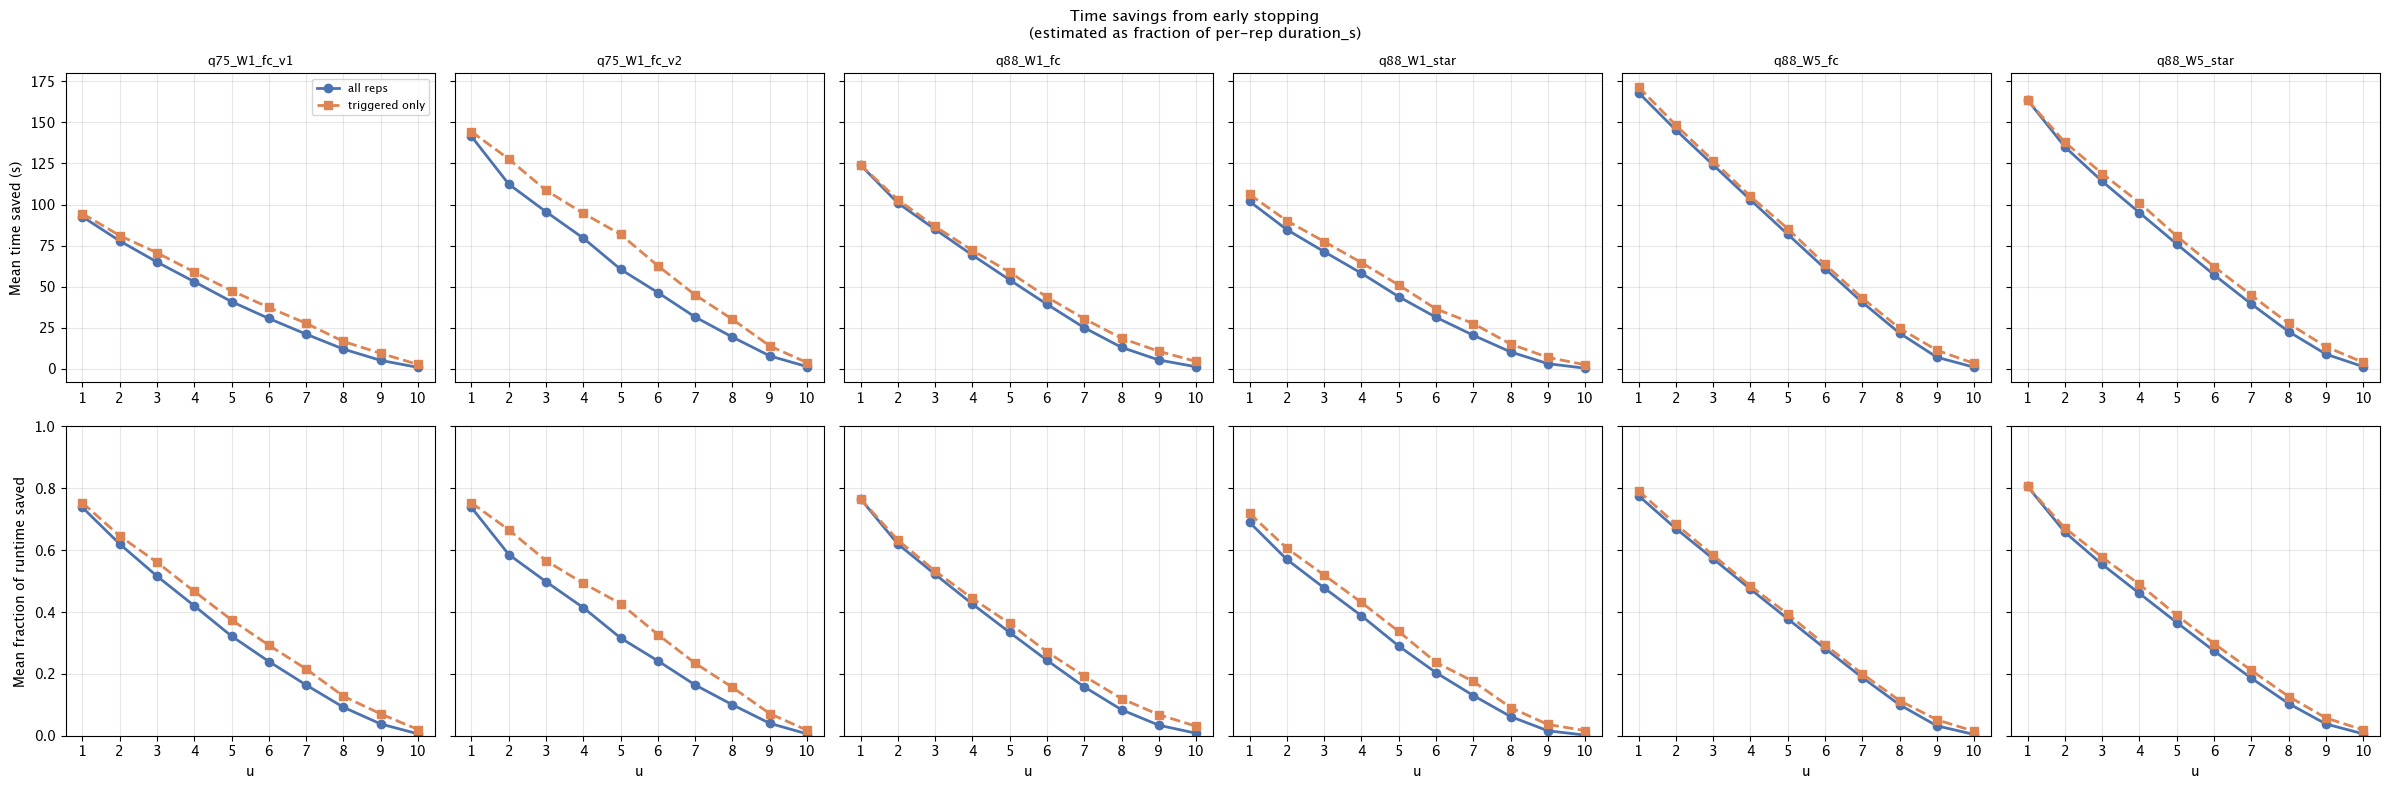
\includegraphics[width=0.75\linewidth]{figures/time_savings.png}
    \caption[Runtime saved by early stopping threshold]{Mean fraction of runtime saved by early stopping as a function of
    the threshold $u$. Solid line: all repetitions. Dashed line: only
    repetitions that triggered stopping. At $u = 3$ the saving is roughly
    $50\,\%$ per repetition.}
    \label{fig:time_savings}
\end{figure}

\paragraph{Output structure (fix, full \arguephase{}/\updatephase{}).}
The structured output is the measurement apparatus, not engineering taste.
Private reasoning and confidence versus the public message enable the
public/private dissociation; the \arguephase{} fields structure the deliberation
(the influence graph for dominance detection is built from vote adoptions, not the
draft text; \autoref{sec:method}); and the vote-stability rule separates argumentation
from belief update so they can be measured independently. Structured outputs are
the norm in serious MAD work \citep{liang2024encouraging, he2025dimo}.

\paragraph{Cooperativeness (fix, cooperative).}
\citet{liang2024encouraging} identify the operational sweet spot: a modest level
of tit-for-tat is required, with pure cooperation collapsing into
Degeneration-of-Thought and pure adversarial framing preventing convergence. Our
defense/challenge/question scaffold implements modest tit-for-tat while \updatephase{} phase
belief update leaves room for convergence.

\paragraph{Synchrony (fix, parallel-synchronous).}
\citet{du2024improving} establish synchronous simultaneous-talk as the canonical
MAD protocol, also adopted by \citet{liu2024groupdebate}. Synchronous execution
with randomised peer-message order also removes agent-order position effects that
would otherwise confound dominance detection.

\paragraph{Model selection (fix, homogeneous mid-tier).}
We fix a single homogeneous model, \texttt{mistral-medium-instruct}, to isolate topology
and memory effects from capability-asymmetry effects: \citet{wynn2025talk} document
that models shift from correct to incorrect answers under peer pressure, producing
dominance-like dynamics attributable to conformity. A homogeneous baseline ensures
any observed dominance is structural rather than capability-driven; heterogeneous
setups are reserved as an ablation. This choice is further supported by evidence
that mixed-model teams within the same capability tier do not systematically
outperform the best homogeneous member and exhibit comparable modal sycophancy
rates, suggesting heterogeneity alone does not dissolve the dynamics under study
\citep{bertalanic2026costofconsensus}.

\paragraph{Sampling temperature (fix at $0.7$, reasoning disabled).}
Deterministic decoding collapses MAD into voting among identical samples, and
\citet{zhu2026demystifying} show the homogeneous deterministic case cannot improve
over a single agent. We use temperature $0.7$ with reasoning disabled to obtain
diverse yet focused outputs without chain-of-thought token overhead. An ablation
comparing $T = 0.4$ against $T = 0.7$ in a comparable debate protocol found that
the lower temperature increased the modal sycophancy rate by $6.2$ percentage
points \citep{bertalanic2026costofconsensus}, providing external support for
the higher-temperature choice.

\paragraph{Tool access (defer).}
For GPQA-Diamond, tools would push single-agent accuracy toward the ceiling and
remove dynamical headroom, introduce non-reproducibility through web search, and
violate the Google-proof design rationale of \citet{rein2024gpqa}.

\paragraph{Compute budget.}
Reliable motif detection requires $R = 30$--$50$ repetitions per configuration:
bistability needs enough samples to surface both attractor basins, limit cycles
enough trajectories to confirm period-$\geq 2$ structure, and dominance
estimators statistical power. At $\approx 25$\,s per repetition, the naive cost of
the full grid on all 198 GPQA-Diamond tasks would be $198 \times 6 \times R \times
25$\,s, i.e.\ $\approx 248$\,h ($\approx 10.3$ days) at $R = 30$ and $\approx 413$\,h
($\approx 17.2$ days) at $R = 50$. The two-phase difficulty-based procedure of
\autoref{sec:setup:design} reduces this to $\approx 29$\,h by running the full
grid only on promoted Tier-3 tasks, while the screening pass still yields
prevalence estimates across the broader task set.
